%
% 公立はこだて未来大学卒業研究中間報告書[情報システム/高度ICTコース]
%
%         ファイル名:"midterm_report.tex"
%
\documentclass[10pt,a4paper]{jsarticle}
\usepackage{funinfosys}
\usepackage[dvipdfmx]{graphicx}
\usepackage{url}

\bibliographystyle{junsrt}	

\author{% 
b1014120 永井陽太\\指導教員 : 松原克弥
}
\course{Advanced ICT Course} %% 高度ICTコースの場合はこちらを使用
\title{教室PCの余剰資源を活用した学内向けオープンクラウドの構築}
\etitle{Implementing an Open Cloud System with Idled Classroom PCs}
\eauthor{Yota Nagai}
\abstract{情報系学科大学では,演習活動の高度化により,学生が実践的な開発を行うようになってきている.
それに伴い,大学に求められる情報基盤も高度になってきており,クラウドコンピューティングが大学に導入されるようになってきている.
しかし,クラウドコンピューティングをオンプレミスに学内に構築する場合,情報基盤センターを持たない大学では,
高価なサーバ機の購入やサーバ管理室を用意する等初期投資が大きくなってしまう.
一方,BYOD等の普及により,講義以外では教室PCが利用されなくなってきている.
そこで,本研究では教室PCの余剰計算資源を活用し学内にクラウドコンピューティングを実現する方法を提案する.
教室PCの死活監視,定期的なバックアップの作成,負荷分散及び一時停止等の機構を実装することによって,
講義に影響を出さずに教室PCを活用する方法を提案する.
}
\keywords{クラウド, 仮想化}
\eabstract{
At universities of the Department of Information Systems, students are beginning to develop practical development by advancement of exercise activities. Along with that, the information infrastructure required for universities is getting higher, and cloud computing has been introduced to universities. However, when building cloud computing on-premises, initial investment such as purchasing expensive server machines and preparing a server management room increases at universities that do not have an information infrastructure center. On the other hand, due to the popularization of BYOD, classroom PCs are no longer used except for lectures. Therefore, in this research, we propose a method to realize cloud computing in campus utilizing surplus computing resources of classroom PC. We propose a method to utilize classroom PC without affecting lecture by implementing mechanisms such as alive monitoring of classroom PC, creation of regular backup, load balancing and temporary stop.	
}
\ekeywords{Cloud, Virtualization}
%\renewcommand{\baselinestretch}{0.98}
\begin{document}
\maketitle
%\vspace*{-.5cm}

\section{はじめに}
\subsection{背景}
近年,クラウド化の時代と言われるほど,あらゆる組織でクラウドコンピューティングが導入されている\cite{academiccloud}.
クラウドコンピューティング導入の動きは,大学においても例外ではない.
平成28年度に文部科学省によって実施された情報基盤実態調査によると,日本の大学の80.6\%が情報システムをクラウド化していると報告されている\cite{SurveyOnActualStateOfAcademicInformationInfrastructure}.
また,近年の情報系学科の大学では,実践的な演習活動を行うようになってきており\cite{practicalict},
学生1人に対して複数台の計算機が利用できる環境を提供することが大学に求められてきている.
\par 大学がクラウドコンピューティングを導入する方法としては,
\begin{enumerate}
	\item 商用クラウドサービスの利用
	\item オンプレミスなプライベートクラウドの構築
\end{enumerate}
という2つの方法が存在するが,
商用のクラウドサービスを利用する場合,サービスの利用料に応じて料金が発生する従量課金制は大学の予算制度との相性が悪い.
また,学内にプライベートクラウドを構築する場合は,高価なサーバ機が必要となり,多大な初期投資が必要である.
\par 一方,情報系学科大学においてはBYODが普及しており,学生1人1人が個人で計算機を持つことが当たり前になってきている.
そのため,統一の演習環境として用意されている教室PCがあまり利用されておらず,有効に活用されていない.
\par また,近年はオープンクラウドと呼ばれる,オープンソースベースのクラウド基盤が普及してきており
クラウドの構築が以前よりも比較的容易になってきている.

\subsection{提案システム}
本研究では,教室PCの余剰資源を活用した学内向けオープンクラウドの構築を試みる.
大学内の教室PCを計算資源の対象とすることで,技術的課題の洗い出しと有効性を確かめる.
\par 提案するシステムは,大学の講義等によって,教室PCが利用され,クラウドの計算資源の状態が動的に変化するという課題がある.
そこで,以下の4つを実現することで上記の課題に対処する.
\begin{itemize}
	\item 計算機として利用できる教室PCを動的に管理する仕組み
	\item 定期的に仮想インスタンスのバックアップを作成する仕組み
	\item 仮想インスタンスのライブマイグレーションを行う仕組み
	\item 利用率の低い仮想インスタンスの一時停止及び再開の仕組み
\end{itemize}

\par 本提案が実現することで,クラウド構築の際の初期投資を抑えながら,
学生に対して1人複数台の計算機を提供できる環境の構築が可能になる
という効果が期待される.

% \par 以降,第2章では,現在の大学教育機関におけるクラウドサービス利用の現状について述べる.
% 第3章で,教室PCを利用した学内オープンクラウドを実現するための技術的課題を示し,その解決方法について論じる.
% 第4章では,実装状況について述べる.第5章では,まとめと今後の課題について述べる.

\begin{figure*}[t]
	\centering
	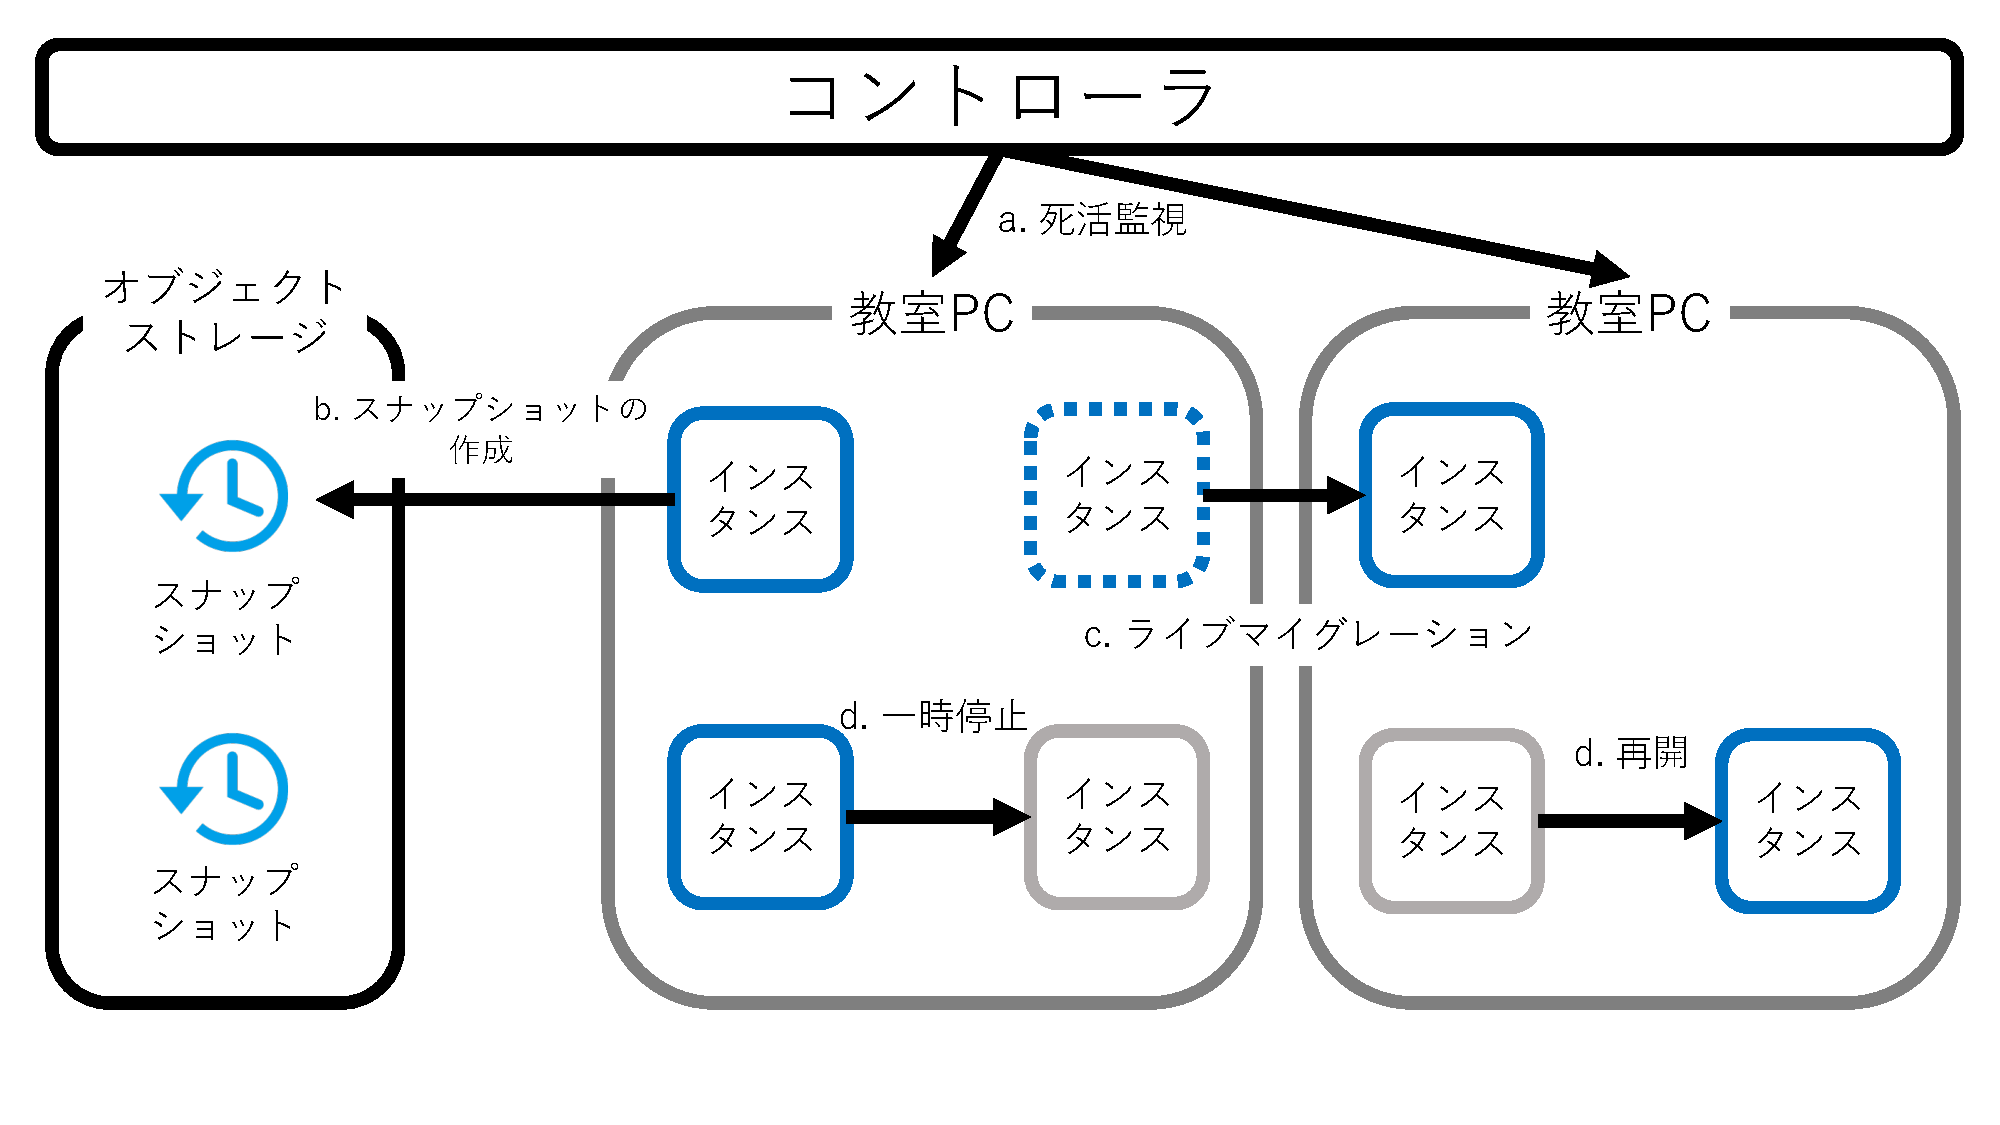
\includegraphics[scale=0.35]{graph1.pdf}
	\label{fig:graph1}
	\begin{center}図1 システムの概要\end{center}
\end{figure*}

\section{大学におけるクラウド利用の欠点及び現状}
\subsection{商用クラウドサービスの欠点}
商用のクラウドサービスを利用する場合の欠点としては,
\begin{enumerate}
	\item 商用クラウドサービスで一般的な従量課金制が大学の予算制度と相性が悪い
	\item 学内ですでに展開されているサービスとの連携が難しくなる
\end{enumerate}
以上の2点が挙げられる.
\subsection{プライベートクラウドの欠点}
プライベートクラウドとは組織内の独自の環境で構築・運用されているクラウドシステムのことである.
プライベートクラウドを利用する際の欠点としては,
\begin{enumerate}
	\item 構築の際に,高価なサーバ機が必要になったり,サーバを設置する環境を整えたりする等の多大な初期投資が必要になる
	\item 組織内に設置したサーバに障害が発生した場合に備えて,障害に対処するサポート体制を整備するための人的なコストがかかる
\end{enumerate}
以上の2点が挙げられる.

\subsection{大学の既存環境と問題点}
現在の情報系学科大学では実践的講義が取り入れられるようになってきており,
クライアントサーバモデルのシステムの構築,
IoTデバイスでセンシングしたデータを集約するためのサーバの構築,
他のWebアプリケーションをネットワークを通して連携するシステムの構築を行うようになってきている.
これらのシステム構成を実現するためには学生1人に対して1台の計算機が提供される環境では不十分になってきている.
したがって,近年の情報系学科大学には学生1人に対して複数台の計算機を提供できる環境を整備することが求められている.
\par 一方,現在の大学では,BYODが普及しており,学生1人1人が個人で専用の計算機を所持している.
東京農工大学では2016年度から完全なBYOD化が実現されている\cite{nokodai}.
BYODの普及により,現在は演習用の教室PCの利用が減ってきている.
しかし,BYODの普及によって学生が持参してくるPCが多様化し,
学生がどのようなPCを持ってくるかわからない状況になっている.
このような状況下では,統一の演習環境が必要になるのでPC教室を撤廃することは難しい.
つまり,教室PCには余剰な計算資源が存在しており,活用されていないという問題がある.

\section{提案するクラウドについて}
% 学内クラウドは止まっても仕方ない,教室PCを利用してクラウドが構築できる事実が素晴らしい
本章では,教室PCの余剰資源を活用したクラウドを実現するにあたり,課題と解決方法について述べる.
\subsection{技術的課題}
\subsubsection{教室PCの予期せぬ停止}
教室PCは学内の任意の人が利用できる状態にあるので,誰でも教室PCの電源を切ることが出来る.
また,自然災害等の外的要因によって,教室PCが停止してしまう可能性が存在する.
教室PCの意図せぬ停止によって,以下の問題が生じる.
\begin{itemize}
	\item クラウドの計算資源として利用できなくなる
	\item 稼働中の仮想インスタンスのデータが消失してしまう可能性が存在する
\end{itemize}
\subsubsection{教室PCの利用による計算資源の枯渇}
クラウドの計算資源として教室PCが利用されていることで教室PCの動作が重くなり,講義に影響がでる可能性がある.
加えて,学内に存在する教室PCのほとんどが講義によって利用されてしまい,計算資源が枯渇する可能性がある.

\subsection{実現手法}
本システムはオープンソースのクラウド基盤であるOpenStack\cite{openstack}の利用及び追加の機構の実装によって実現する.
OpenStackはマイクロサービスアーキテクチャを採用しており,6つのコアサービスによって構成されている.
6つのコアサービスの内,技術的課題の解決に関わるコアサービスNovaとSwiftについて説明する.
\begin{itemize}
	\item Nova:仮想インスタンスを立ち上げる為の計算機の管理及び仮想インスタンスの管理を担っている.計算機の情報を,随時コントローラに送信することで,計算機の死活監視や,仮想インスタンスを立ち上げる最適な計算機を決定する役割も担っている.
	\item Swift:イメージファイルやメディアファイル等のオブジェクトを保存する為のストレージの提供及び管理を担っている.レプリケーションにも対応しており,障害への対策も可能である.
\end{itemize}
\subsubsection{教室PCの死活監視と定期的なバックアップ}
計算資源として利用できる教室PCが変化問題には,Novaの死活監視によって対応が可能である(図1のa).
稼働中の仮想インスタンスのデータが消失してしまう可能性については,
定期的に仮想インスタンスのスナップショットを作成し,オブジェクトストレージSwiftに保存することで対応する(図1のb).
\subsubsection{教室PCの負荷分散及び仮想インスタンスの一時停止}
講義による教室PCの利用は講義時間割から予測が可能なので,講義が始まる前に利用されない教室PCへ仮想インスタンスをライブマイグレーションすることで対応が可能である(図1のc).
また,講義によって計算資源が枯渇してしまう問題に対しては,一定期間のアクセス数等の仮想インスタンスの利用状況から
もっとも利用されていない仮想インスタンスを決定するアルゴリズムを考案し,そのアルゴリズムによって決定されたインスタンスを一時停止状態にすることで対応が可能である(図1のd).

\section{実装状況}
\subsection{研究室におけるクラウドの構築}
本学における教室PCのOSはmacOSとWindowsが存在する.
したがって,本学におけるクラウドの実装としては,macOSとWindowsが動作している計算機を対象とする.
現在はプロトタイプとして,研究室内にOpenStackを利用してプライベートなクラウドを構築している段階である.
クラウドの計算資源として,まずはCentOS7を利用した後,macOS High Sierraを追加する予定である.
その後は,macOS High Sierra上の仮想インスタンスの定期的なバックアップの作成
及び仮想インスタンスの一時停止と再開の機構を実装する予定である.

\section{おわりに}
\subsection{まとめ}
本研究では,教室PCの余剰資源を活用した学内向けオープンクラウドの実現方式の提案を行った.
教室PCの不安定な計算資源に対して,
計算機の死活監視,仮想インスタンスのバックアップ,
仮想インスタンスのライブマイグレーション及び
利用順位付けアルゴリズムによる仮想インスタンスの一時停止・再開
等の機構を実装したクラウドの構築の検討を行った.
提案するシステムがもたらす効果として,
学内の余剰計算機を用いることでプライベートクラウド構築の欠点である初期投資を抑えながら,
学生に対して1人複数台の計算機を提供する環境の構築が可能になることが見込める.
\subsection{今後の課題}
今後は,有限な計算資源を学生全体に平等に提供するため,
学生1人に対し,具体的に何台計算機を提供するのか決定する必要がある.
また,どのように学内の認証機構との連携を行うのか,考慮する必要がある.
さらに,学生が仮想インスタンスを操作するためのWebUIをOpenStackのデフォルトの状態から,学生が使いやすいUIを検討する必要がある.

\bibliography{ref.bib}
\end{document}
%
%
% EOF 
